\chapter{Giới thiệu}
\label{chap:intro}

\section{Động lực}

Trong những năm gần đây, hệ sinh thái blockchain đã phát triển nhanh chóng với sự xuất hiện của nhiều nền tảng và ứng dụng phi tập trung (dApp), đặc biệt trong các lĩnh vực như tài chính phi tập trung (DeFi), NFT hay GameFi. Sự đa dạng của các blockchain như Ethereum, BNB Chain, Solana và các giải pháp Layer 2 đã tạo ra một môi trường phong phú nhưng đồng thời cũng dẫn đến sự phân mảnh về tài sản và thanh khoản. Trong bối cảnh đó, nhu cầu tương tác xuyên chuỗi (cross-chain interaction) trở thành một yêu cầu tất yếu, cho phép người dùng di chuyển tài sản và thực hiện giao dịch giữa các blockchain khác nhau.

Các giải pháp phổ biến hiện nay để hỗ trợ tương tác xuyên chuỗi chủ yếu dựa trên cơ chế bridge. Tuy nhiên, các bridge truyền thống tồn tại nhiều hạn chế cả về chi phí, hiệu năng và đặc biệt là bảo mật. Người dùng thường phải thực hiện nhiều giao dịch trên các blockchain khác nhau, dẫn đến chi phí gas cao và nhiều rủi ro. Quan trọng hơn, bridge đã trở thành mục tiêu của nhiều cuộc tấn công nghiêm trọng, gây thiệt hại lớn cho hệ sinh thái. Các sự kiện như Ronin Bridge hack và Wormhole hack cho thấy rõ ràng rằng bridge là một trong những điểm yếu mang tính hệ thống trong kiến trúc blockchain hiện tại.

Song song với đó, khối lượng giao dịch cross-chain liên tục gia tăng, đạt mức hàng tỷ USD mỗi tháng, phản ánh nhu cầu thực tế rất lớn từ phía người dùng. Điều này đặt ra yêu cầu cấp thiết về việc tìm kiếm một mô hình mới có khả năng thay thế hoặc cải thiện các cơ chế bridge hiện tại, nhằm giảm thiểu rủi ro, tối ưu chi phí và nâng cao hiệu năng.

Một hướng tiếp cận tiềm năng cho bài toán tương tác xuyên chuỗi có thể được tìm thấy từ lĩnh vực tài chính truyền thống, cụ thể là mô hình hoạt động của Wise (formerly TransferWise). Thay vì sử dụng các hệ thống trung gian phức tạp như SWIFT để thực hiện chuyển tiền quốc tế, Wise áp dụng cơ chế netting nội bộ nhằm tối ưu hóa dòng tiền giữa các quốc gia.

% TODO: figure - "How TransferWise works" infographic (from the original PDF).
% Place the image file at figures/c1/transferwise.png then uncomment below.
% \begin{figure}[H]
%   \begin{center}
%   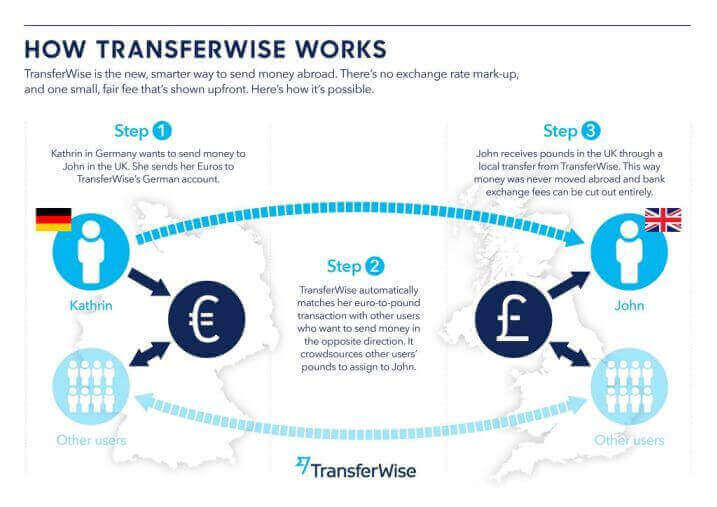
\includegraphics[width=0.8\linewidth]{figures/c1/transferwise}
%   \end{center}
%   \caption{Mô hình hoạt động của TransferWise (Wise) — netting nội bộ giữa các quốc gia}
%   \label{fig:transferwise}
% \end{figure}

Trong mô hình truyền thống, khi một người dùng chuyển tiền từ quốc gia A sang quốc gia B, dòng tiền thực tế phải đi qua nhiều tổ chức trung gian, dẫn đến chi phí cao và thời gian xử lý kéo dài. Ngược lại, Wise duy trì thanh khoản tại nhiều quốc gia và thực hiện việc đối soát các dòng tiền đối ứng trong hệ thống. Cụ thể, nếu tồn tại một người dùng chuyển tiền từ A sang B và một người khác chuyển từ B sang A, hệ thống có thể ghép nối hai giao dịch này và chỉ cần điều chỉnh số dư nội bộ, thay vì thực hiện hai giao dịch xuyên biên giới độc lập. Nhờ đó, lượng tiền thực sự cần di chuyển giữa các quốc gia được giảm thiểu đáng kể.

Từ góc nhìn này, có thể nhận thấy một sự tương đồng đáng kể giữa hệ thống tài chính truyền thống và hệ sinh thái blockchain hiện nay. Mỗi blockchain có thể được xem như một ``quốc gia'' độc lập, với tài sản và thanh khoản được quản lý riêng biệt. Các giao dịch cross-chain, về bản chất, tương tự như các giao dịch xuyên biên giới trong tài chính truyền thống, khi tài sản cần được chuyển từ một hệ thống này sang một hệ thống khác. Dựa trên sự tương đồng đó, nghiên cứu này đề xuất việc áp dụng tư duy của cơ chế netting vào bài toán cross-chain. Thay vì phụ thuộc hoàn toàn vào các bridge để chuyển tài sản trực tiếp giữa các blockchain, hệ thống có thể khai thác các nhu cầu giao dịch đối ứng của người dùng và thực hiện việc ghép nối các \textit{intent} tương thích. Khi đó, phần lớn các giao dịch có thể được xử lý thông qua cơ chế matching nội bộ, trong khi nhu cầu chuyển tài sản thực tế giữa các chain được giảm thiểu.

Cách tiếp cận này không chỉ giúp tối ưu hóa chi phí và độ trễ mà còn có tiềm năng giảm thiểu đáng kể rủi ro bảo mật, do hạn chế sự phụ thuộc vào các bridge --- vốn là điểm yếu phổ biến trong các hệ thống cross-chain hiện tại. Qua đó, mô hình được đề xuất mở ra một hướng đi mới, trong đó việc tương tác giữa các blockchain được thực hiện một cách hiệu quả hơn thông qua cơ chế điều phối và đối soát, thay vì di chuyển tài sản trực tiếp.

\section{Khái niệm cơ bản \& cơ sở lý thuyết}

Để xây dựng và phân tích hệ thống giao dịch xuyên chuỗi dựa trên intent, cần làm rõ một số khái niệm và mô hình nền tảng trong cả lĩnh vực blockchain và tài chính truyền thống. Các khái niệm này không chỉ giúp hiểu cách các hệ thống hiện tại vận hành mà còn làm rõ những hạn chế, từ đó tạo cơ sở cho hướng tiếp cận được đề xuất trong nghiên cứu này.

Các khái niệm và cơ sở lý thuyết chính bao gồm:

\begin{itemize}
    \item \textbf{Cross-chain bridge}: là cơ chế cho phép chuyển tài sản hoặc dữ liệu giữa các blockchain khác nhau. Các bridge phổ biến thường hoạt động theo mô hình \textit{lock-and-mint} (khóa tài sản trên chain nguồn và phát hành tài sản đại diện trên chain đích) hoặc dựa trên liquidity pool. Mặc dù cho phép hiện thực hóa giao dịch cross-chain, các mô hình này đòi hỏi sự tin cậy vào smart contract, các bên trung gian như relayer hoặc validator, từ đó làm gia tăng rủi ro bảo mật.
    \item \textbf{Cross-chain interaction}: là khái niệm tổng quát bao hàm tất cả các hình thức tương tác giữa các blockchain, bao gồm chuyển tài sản, message và đồng bộ trạng thái. Đây là bài toán phức tạp do sự khác biệt về kiến trúc và cơ chế đồng thuận giữa các chain, đồng thời là nền tảng cho các ứng dụng đa chuỗi hiện đại.
    \item \textbf{Intent-based execution}: là mô hình trong đó người dùng chỉ cần mô tả mục tiêu mong muốn thay vì các bước thực hiện cụ thể. Hệ thống sẽ sử dụng các tác nhân trung gian (solver) để tìm và thực thi phương án tối ưu. Một ví dụ tiêu biểu là CoW Protocol, nơi các lệnh giao dịch được gom lại và xử lý thông qua cơ chế batch auction nhằm tận dụng sự trùng khớp giữa các nhu cầu giao dịch.
    \item \textbf{Atomic swap và HTLC (Hashed Timelock Contract)}: là cơ chế cho phép hai bên trao đổi tài sản giữa các blockchain mà không cần tin cậy lẫn nhau. HTLC sử dụng kết hợp hashlock và timelock để đảm bảo rằng giao dịch chỉ được thực hiện khi cả hai bên đều hoàn thành nghĩa vụ. Tuy nhiên, mô hình này gặp hạn chế về khả năng mở rộng và khó áp dụng trong các hệ thống nhiều bên.
    \item \textbf{Mô hình tài chính truyền thống (SWIFT, Wise)}:
    \begin{itemize}
        \item SWIFT là hệ thống truyền thông giữa các ngân hàng, hỗ trợ chuyển tiền quốc tế nhưng phụ thuộc vào nhiều trung gian, dẫn đến chi phí cao và độ trễ lớn.
        \item Wise (formerly TransferWise) áp dụng cơ chế \textit{netting nội bộ}, cho phép đối soát các dòng tiền đối ứng và giảm thiểu việc chuyển tiền xuyên biên giới thực tế.
    \end{itemize}
\end{itemize}

\subsection*{Các pattern bridge phổ biến}
\addcontentsline{toc}{subsection}{Các pattern bridge phổ biến}

Các bridge có thể được phân loại dựa trên cách mà chain đích xác minh trạng thái hoặc giao dịch từ chain nguồn:

\begin{itemize}
    \item \textbf{State validating protocols}: là mô hình trong đó chain đích có thể xác minh trực tiếp trạng thái của chain nguồn dựa trên các giả định bảo mật của blockchain gốc. Mô hình này thường xuất hiện trong các bridge giữa Layer 1 và Layer 2, nơi Layer 1 đóng vai trò là ``source of truth''. Nhờ đó, mức độ bảo mật cao vì không cần tin tưởng bên thứ ba, nhưng chi phí tính toán và triển khai thường lớn.
    \item \textbf{Consensus verifying protocols}: trong mô hình này, chain đích xác minh rằng một giao dịch trên chain nguồn đã được hoàn tất thông qua việc kiểm chứng cơ chế đồng thuận. Điều này thường yêu cầu các bằng chứng (proof) về block hoặc transaction, giúp đảm bảo tính đúng đắn mà không cần tin cậy hoàn toàn vào bên trung gian.
    \item \textbf{Third-party attestation protocols}: là mô hình phổ biến nhất trong thực tế, trong đó một thực thể trung gian (có thể là một validator, một tập hợp multi-signature hoặc một blockchain riêng) xác nhận tính hợp lệ của giao dịch. Ưu điểm là dễ triển khai và hiệu năng cao, nhưng nhược điểm lớn là phụ thuộc vào trust assumption, dẫn đến nhiều rủi ro bảo mật.
    \item \textbf{Optimistic protocols}: dựa trên giả định rằng các giao dịch là hợp lệ trừ khi bị chứng minh ngược lại. Một hoặc nhiều ``watcher'' có thể phát hiện và báo cáo gian lận trong một khoảng thời gian gọi là fraud window. Mô hình này giảm chi phí xác minh ban đầu nhưng yêu cầu cơ chế challenge hiệu quả để đảm bảo an toàn.
\end{itemize}

\subsection*{Các loại hình vận hành phổ biến của bridge}
\addcontentsline{toc}{subsection}{Các loại hình vận hành phổ biến của bridge}

Bên cạnh messaging protocol, bridge còn được phân loại theo cách thức xử lý tài sản và giao dịch giữa các chain:

\begin{itemize}
    \item \textbf{Liquidity networks}: sử dụng các pool thanh khoản trên nhiều chain. Người dùng gửi tài sản vào pool trên chain nguồn và nhận tài sản tương ứng từ pool trên chain đích. Mô hình này không yêu cầu mint tài sản mới mà tận dụng thanh khoản có sẵn, giúp giảm độ trễ và cải thiện trải nghiệm người dùng, nhưng phụ thuộc vào thanh khoản và có thể gặp rủi ro mất cân bằng pool.
    \item \textbf{Token bridges}: hoạt động theo mô hình khóa (lock) hoặc đốt (burn) tài sản trên chain nguồn và phát hành (mint) tài sản tương ứng trên chain đích. Các token được tạo ra trên chain đích thường là tài sản tổng hợp (wrapped asset), đại diện cho quyền sở hữu tài sản gốc. Đây là mô hình phổ biến nhất nhưng cũng là mục tiêu của nhiều cuộc tấn công do tồn tại các thành phần như custodian và debt issuer.
    \item \textbf{Coordination protocols}: không chỉ tập trung vào chuyển tài sản mà còn hỗ trợ tương tác phức tạp giữa các chain, như gọi hàm, truyền dữ liệu hoặc đồng bộ trạng thái. Mô hình này cho phép xây dựng các ứng dụng đa chuỗi (cross-chain dApps), nhưng đồng thời làm tăng đáng kể độ phức tạp của hệ thống.
\end{itemize}

Từ các khái niệm trên, có thể nhận thấy rằng các hệ thống hiện tại, dù trong blockchain hay tài chính truyền thống, đều phải đối mặt với bài toán tối ưu hóa giữa chi phí, hiệu năng và độ an toàn. Đặc biệt, cơ chế netting trong tài chính truyền thống và mô hình intent-based trong blockchain gợi mở khả năng kết hợp để xây dựng một hệ thống cross-chain hiệu quả hơn, trong đó việc ghép nối các nhu cầu giao dịch có thể thay thế cho việc di chuyển tài sản trực tiếp giữa các chain.

\section{Phát biểu bài toán}

Nghiên cứu này tập trung vào việc xây dựng một hệ thống hỗ trợ giao dịch xuyên chuỗi dựa trên mô hình intent, với mục tiêu giảm thiểu sự phụ thuộc vào bridge truyền thống.

\subsection{Đầu vào}

Đầu vào của hệ thống là một tập hợp các \textit{intent order} do người dùng cung cấp, trong đó mỗi intent biểu diễn nhu cầu chuyển tài sản từ một blockchain nguồn sang một blockchain đích. Mỗi intent không mô tả chi tiết quá trình thực hiện mà chỉ xác định các tham số mục tiêu mà hệ thống cần thỏa mãn.

Cụ thể, một intent được đặc trưng bởi các thông tin sau:

\begin{itemize}
    \item \textbf{Source chain}: blockchain nơi tài sản ban đầu được nắm giữ
    \item \textbf{Destination chain}: blockchain mà người dùng mong muốn nhận tài sản
    \item \textbf{Amount}: số lượng tài sản cần chuyển
    \item \textbf{Deadline}: thời hạn mà giao dịch cần được hoàn tất
    \item \textbf{Incentive}: phần thưởng dành cho các tác nhân (solver) tham gia xử lý intent; trong trường hợp bằng 0, hệ thống chỉ thực hiện matching ngang hàng qua p2p network
\end{itemize}

Trong phạm vi nghiên cứu này, tài sản được giả định là USDC trên chain nguồn nhằm đơn giản hóa việc phân tích và tập trung vào cơ chế matching xuyên chuỗi.

Các intent trong hệ thống có thể tồn tại độc lập hoặc có mối quan hệ đối ứng với nhau. Khi xuất hiện các intent có thể ghép nối, hệ thống cần xác định các cặp hoặc nhóm intent tương thích để thực hiện matching, từ đó giảm thiểu nhu cầu sử dụng bridge và tối ưu hóa chi phí giao dịch.

\subsection{Đầu ra}

Đầu ra của hệ thống là trạng thái trong đó người dùng nhận được tài sản tương ứng trên blockchain đích, thỏa mãn các điều kiện đã đặt ra trong intent ban đầu. Cụ thể, người dùng cần nhận được một lượng USDC trên chain đích không thấp hơn giá trị yêu cầu, trong khoảng thời gian cho phép.

Hệ thống cần đảm bảo rằng quá trình thực hiện giao dịch là chính xác, an toàn và hiệu quả, đồng thời tối ưu hóa việc sử dụng tài nguyên và thanh khoản trong toàn bộ hệ thống.

\subsection{Giải pháp tồn tại}

Để đánh giá tổng quan các kiến trúc bridge hiện nay, tiến hành phân loại các bridge dựa trên các pattern bridge trong mục 1.2: (i) cơ chế truyền thông giữa các chain (communication protocol) và (ii) loại hình vận hành (bridge type). Kết quả được biểu diễn dưới dạng một bảng, trong đó các cột tương ứng với các messaging protocol (state validating, consensus verifying, third-party attestation, optimistic), còn các hàng tương ứng với các loại bridge (liquidity network, token bridge, coordination protocol).

% TODO: figure - bridge taxonomy matrix (from the original PDF).
% Place image at figures/c1/bridge-taxonomy.png and uncomment below.
% \begin{figure}[H]
%   \begin{center}
%   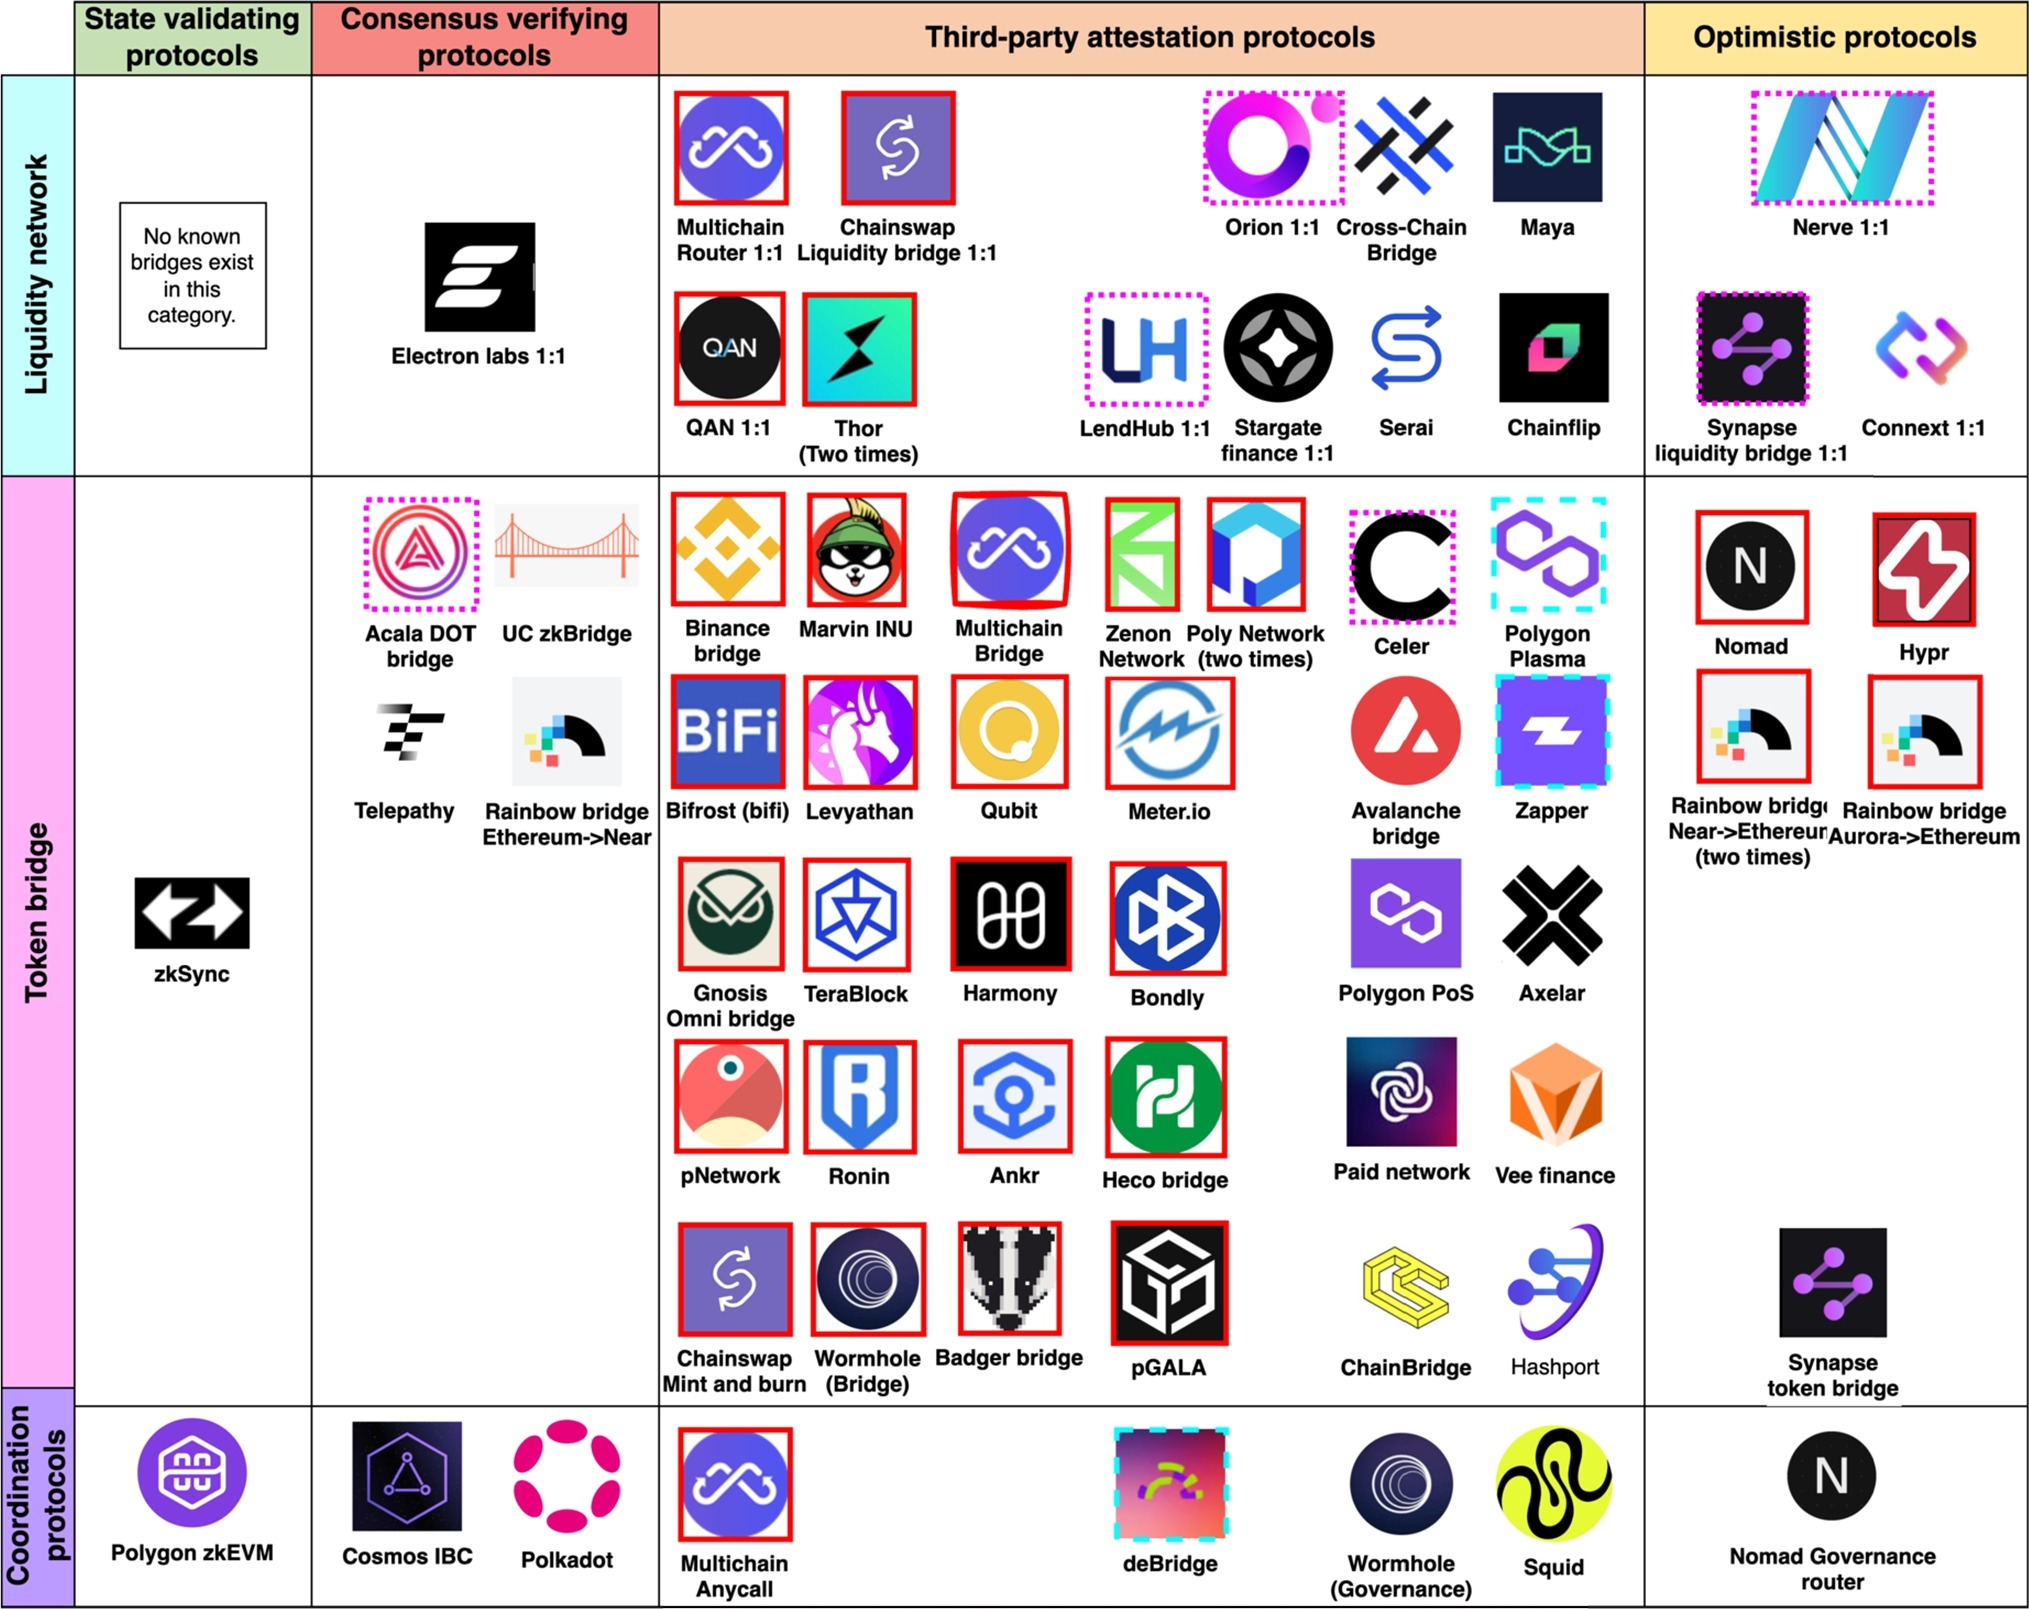
\includegraphics[width=\linewidth]{figures/c1/bridge-taxonomy}
%   \end{center}
%   \caption{Phân loại các bridge theo messaging protocol và type of operation, đánh dấu trạng thái bảo mật}
%   \label{fig:bridge-taxonomy}
% \end{figure}

Trong biểu đồ này, mỗi bridge được đánh dấu theo trạng thái bảo mật: các bridge bị tấn công được viền đỏ, các bridge có lỗ hổng đã được phát hiện nhưng chưa bị khai thác được viền xanh lam nét đứt, và các trường hợp nằm ngoài phạm vi nghiên cứu được đánh dấu bằng viền hồng. Cách biểu diễn này cho phép quan sát trực quan mối quan hệ giữa kiến trúc bridge và mức độ rủi ro bảo mật.

Từ kết quả phân loại, có thể rút ra một số nhận định quan trọng về các mô hình bridge hiện tại. Trước hết, phần lớn các bridge trong thực tế được xây dựng dựa trên \textbf{third-party attestation protocols}. Đây là mô hình mà một hoặc một nhóm validator hoặc relayer trung gian xác nhận các giao dịch cross-chain. Các bridge tiêu biểu sử dụng mô hình này bao gồm Binance Bridge, Wormhole, Multichain hay Ronin Network. Ưu điểm của cách tiếp cận này là dễ triển khai và có hiệu năng cao, tuy nhiên nó phụ thuộc mạnh vào giả định tin cậy đối với các thực thể trung gian. Thực tế cho thấy đây cũng chính là điểm yếu bảo mật lớn nhất. Nhiều vụ tấn công nghiêm trọng đã xảy ra trên các bridge thuộc nhóm này, tiêu biểu như Ronin Bridge hack với thiệt hại khoảng 625 triệu USD do attacker kiểm soát majority validator, hay Wormhole hack với khoảng 320 triệu USD do lỗi xác minh chữ ký. Ngoài ra, Binance Bridge cũng từng bị khai thác với thiệt hại hàng trăm triệu USD do forged proof. Các ví dụ này cho thấy rằng khi trust assumption bị phá vỡ, toàn bộ hệ thống bridge có thể bị khai thác trực tiếp. Do đó, có thể kết luận rằng \textbf{third-party attestation là mô hình phổ biến nhất nhưng cũng là yếu nhất về mặt bảo mật}.

Tương tự, các \textbf{optimistic protocols} cũng tồn tại những rủi ro đáng kể. Một số bridge như Nomad hay Rainbow Bridge áp dụng mô hình này, trong đó giao dịch được coi là hợp lệ mặc định và chỉ bị hủy nếu có fraud proof. Tuy nhiên, trong vụ tấn công Nomad năm 2022, một lỗi khởi tạo đã khiến bất kỳ giao dịch nào cũng được coi là hợp lệ, dẫn đến việc hàng trăm triệu USD bị rút khỏi hệ thống. Điều này cho thấy rằng mặc dù optimistic bridge giảm chi phí xác minh ban đầu, nó phụ thuộc mạnh vào cơ chế challenge và watcher, và khi các cơ chế này thất bại, hệ thống có thể bị khai thác trên diện rộng.

Đối với \textbf{consensus verifying protocols}, đây là một hướng tiếp cận có tiềm năng cao về mặt bảo mật vì chain đích có thể xác minh tính hợp lệ của giao dịch dựa trên bằng chứng từ cơ chế đồng thuận của chain nguồn. Một số ví dụ liên quan đến hướng này có thể kể đến các thiết kế relay chain hoặc light client-based bridge trong hệ sinh thái như Cosmos IBC hoặc các nghiên cứu về zkBridge. Tuy nhiên, số lượng bridge thực tế áp dụng mô hình này vẫn còn hạn chế. Nguyên nhân chủ yếu là do chi phí triển khai cao, yêu cầu xác minh phức tạp (ví dụ: light client verification hoặc zk-proof), và khó tích hợp với các blockchain không tương thích. Do đó, mặc dù có ưu điểm về bảo mật, \textbf{consensus verifying chưa được áp dụng rộng rãi trong thực tế}.

Cuối cùng, \textbf{state validating protocols} được xem là mô hình có mức độ bảo mật cao nhất, khi toàn bộ trạng thái của chain nguồn có thể được xác minh trực tiếp trên chain đích. Các bridge giữa Layer 1 và Layer 2 như Optimism hoặc zkSync bridge là ví dụ điển hình, nơi Layer 1 đóng vai trò là nguồn chân lý duy nhất. Tuy nhiên, mô hình này hầu như không được áp dụng cho các bridge giữa các blockchain độc lập do yêu cầu kỹ thuật rất cao, đặc biệt là việc xác minh state hoặc proof một cách hiệu quả. Điều này khiến cho \textbf{state validating có độ an toàn cao nhưng phạm vi ứng dụng còn hạn chế}.

Xét theo góc độ \textbf{type of operation}, có thể nhận thấy rằng phần lớn các bridge hiện nay hoạt động theo mô hình \textbf{token bridge} và \textbf{coordination protocol}. Các bridge như Wormhole, Multichain hay Binance Bridge chủ yếu sử dụng mô hình token bridge với cơ chế lock-and-mint hoặc burn-and-mint. Đây cũng chính là lý do khiến các thành phần như custodian và debt issuer trở thành mục tiêu chính của các cuộc tấn công.

Ngược lại, các \textbf{liquidity network} như ThorChain hoặc một số thiết kế của Across Protocol có cách tiếp cận khác, dựa trên việc sử dụng pool thanh khoản thay vì mint token mới. Mặc dù mô hình này có thể giảm một số rủi ro liên quan đến custodian, nó lại phụ thuộc vào thanh khoản và cơ chế cân bằng giữa các pool, đồng thời chưa chiếm tỷ trọng lớn trong các bridge được khảo sát.

Từ các phân tích trên, có thể thấy rằng các giải pháp bridge hiện tại chủ yếu đánh đổi giữa hiệu năng và bảo mật. Các mô hình phổ biến như third-party attestation đạt được hiệu năng cao nhưng lại dễ bị khai thác, trong khi các mô hình an toàn hơn như consensus verifying hoặc state validating lại khó triển khai và chưa phổ biến. Điều này cho thấy một khoảng trống rõ ràng trong thiết kế hệ thống cross-chain, nơi cần một cách tiếp cận mới có thể giảm phụ thuộc vào trung gian mà vẫn đảm bảo hiệu quả và an toàn.
